\section{Interpretation of Results}
\label{sec:InterpretationOfResults}
%Try to give an interpretation of you results in your answers to the problems.
%Compare results with closed form solution
It can be shown by inserting into the \eqref{eq:Nature1} that 
\begin{align}
	u(x) = 1-(1-e^{-10})x-e^{-10x}
	\label{eq:IntOfResult1a}
\end{align}
is a solution to the differential equation. 
In the figure below ...
\begin{figure}[H]
	\centering
	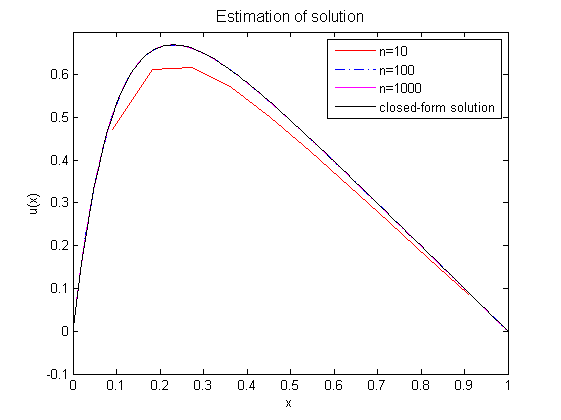
\includegraphics[width=0.8\textwidth]{Figures/estimaition_of_solution.png}
	\caption{Plot of the closed-form solution together with the numerical solution for different n-values. It is evident that the precision of the numerical solution gets better when number of grid points is increased from $n=10$ to $n=100$ and $n=1000$.}
	\label{fig:IntOfResult1}
\end{figure}
From \figref{fig:IntOfResult1} it is easily seen that by increasing the number of grid points from $n=10$ to $n=100$ the precision of the solution is better. 
However, it is not evident from the figure that a further increment of $n$ improves the precision further. 
By zooming in on the figure, it can be seen that an increment of $n$ from 100 to 1000 actually gives a futher improvement to the numerical solution.   
\begin{figure}[H]
	\centering
	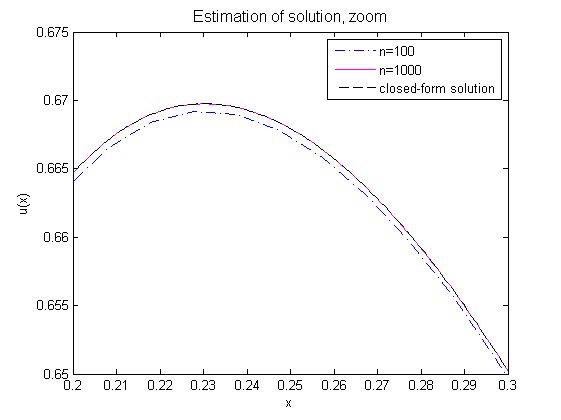
\includegraphics[width=0.8\textwidth]{Figures/estimaition_of_solution_zoom.png}
	\caption{Zoom of \figref{fig:IntOfResult1}. It is seen that a further increment of $n$ from 100 to 1000 actually improves the precision of the result.}
	\label{fig:IntOfResult2}
\end{figure}

%Data for relative error (data in excel sheed) gained from the cpp code
From \figref{fig:IntOfResult1} and \figref{fig:IntOfResult2} it is evident that there is a deviation between the closed-form solution $\v{u}$ and the numerical solution gained by the algorithm made in the project, and that the deviation decreased with increasing number of grid points $n$.
To see how this deviation actually reacts on a change in number of grid points which is directly related to the steplength, consider the relative error $\epsilon_i$ given by
\begin{align}
	\epsilon_i=log_{10}\left(\left|\frac{v_i-u_i}
                 {u_i}\right|\right)
    \label{eq:IntOfResult1}
\end{align}
in which $v_i$ is the i'th element of the numerical solution $\v{v}$ gained by the c++ code described in \secref{sec:DescriptionOfTheAlgorithm}, and $u_i$ is the i'th element of the closed-form-solution $\v{u}$ calculated by the formula EQ with $x=(i+1)h$ as the relation between i and $x$ for steplength $h$.  

\begin{table}[H]
	\centering
  \begin{tabular}{| l | c | c | c |}
    \hline
    $n$		& $h$ 	& $\log(h)$ & $\epsilon_i$ \\ \hline
    10 		& 0.090909 	& -1.04139 & -1.1797 
    \\ \hline
    100 	& 0.009901 	& -2.00432 & -3.08804 
    \\ \hline
    1000 	& 0.000999 	& -3.00043 & -5.08005 
    \\ \hline
	10000 	& 0.000099 	& -4.00004 & -7.07934 
    \\ \hline
    100000 	& $10^{-5}$	& -5	   & -8.888 
    \\ \hline
  \end{tabular}
  \caption{The table shows different relative errors $\epsilon_i$ for different $n$'s corresponding to different steplengths $h$. The steplength $h$ and logarithm to the steplength is calculated in Excel, whilst the relative error $\epsilon_i$ is calculated as in \eqref{eq:IntOfResult1} using the c++ code. When the number of grid points $n$ was increased to 100,000, the precision on the fifth digit of $\epsilon_i$ was lost, which is why only the first four digits of $\epsilon_i$ for $n = 100,000$ are shown in the table.}
  \label{tab:IntOfResult1}
\end{table}

\begin{figure}[H]
	\centering
	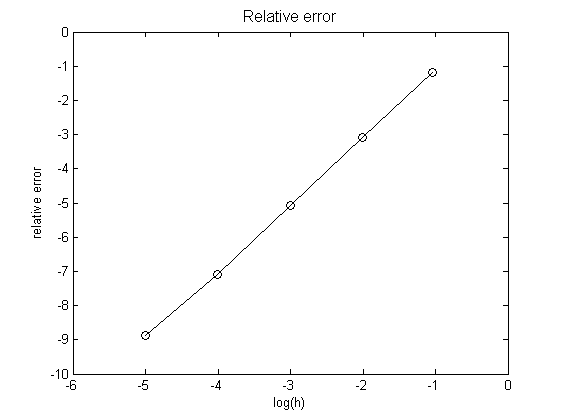
\includegraphics[width=0.8\textwidth]{Figures/relativeerror5.png}
	\caption{Plot of the relative error of the numerical solution to the closed-form solution as a function of the step length. These datapoints are connected by a almost straight line with a slope of approximately 2.}
	\label{fig:IntOfResult2}
\end{figure}
\fxnote{comment on the slope}
